
\begin{appendices}
	
	\begin{centerappendixtitle}
		% use centerappendixtitle if the supplementary materials will cover the entire page
		% input the title as usual then insert \pagebreak right after the title
		\chapter{System Flow Chart}
		\pagebreak
		
		\begin{figure}[h]
			\centering
			\caption{Genetic Algorithm}
			\label{genalgoFlow}
			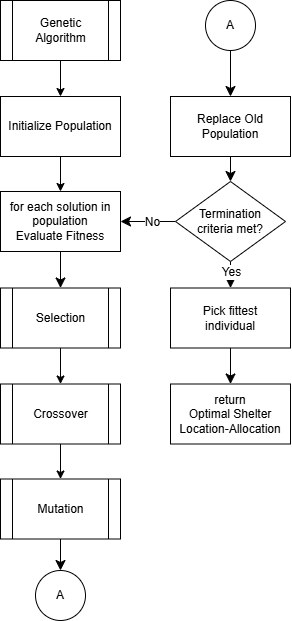
\includegraphics[width=\textwidth,height=\textheight,keepaspectratio]{appendix/Genetic Algorithm Flowchart}
		\end{figure}
		
		\begin{figure}[h]
			\centering
			\caption{Genetic Algorithm - Selection}
			\label{selectFlow}
			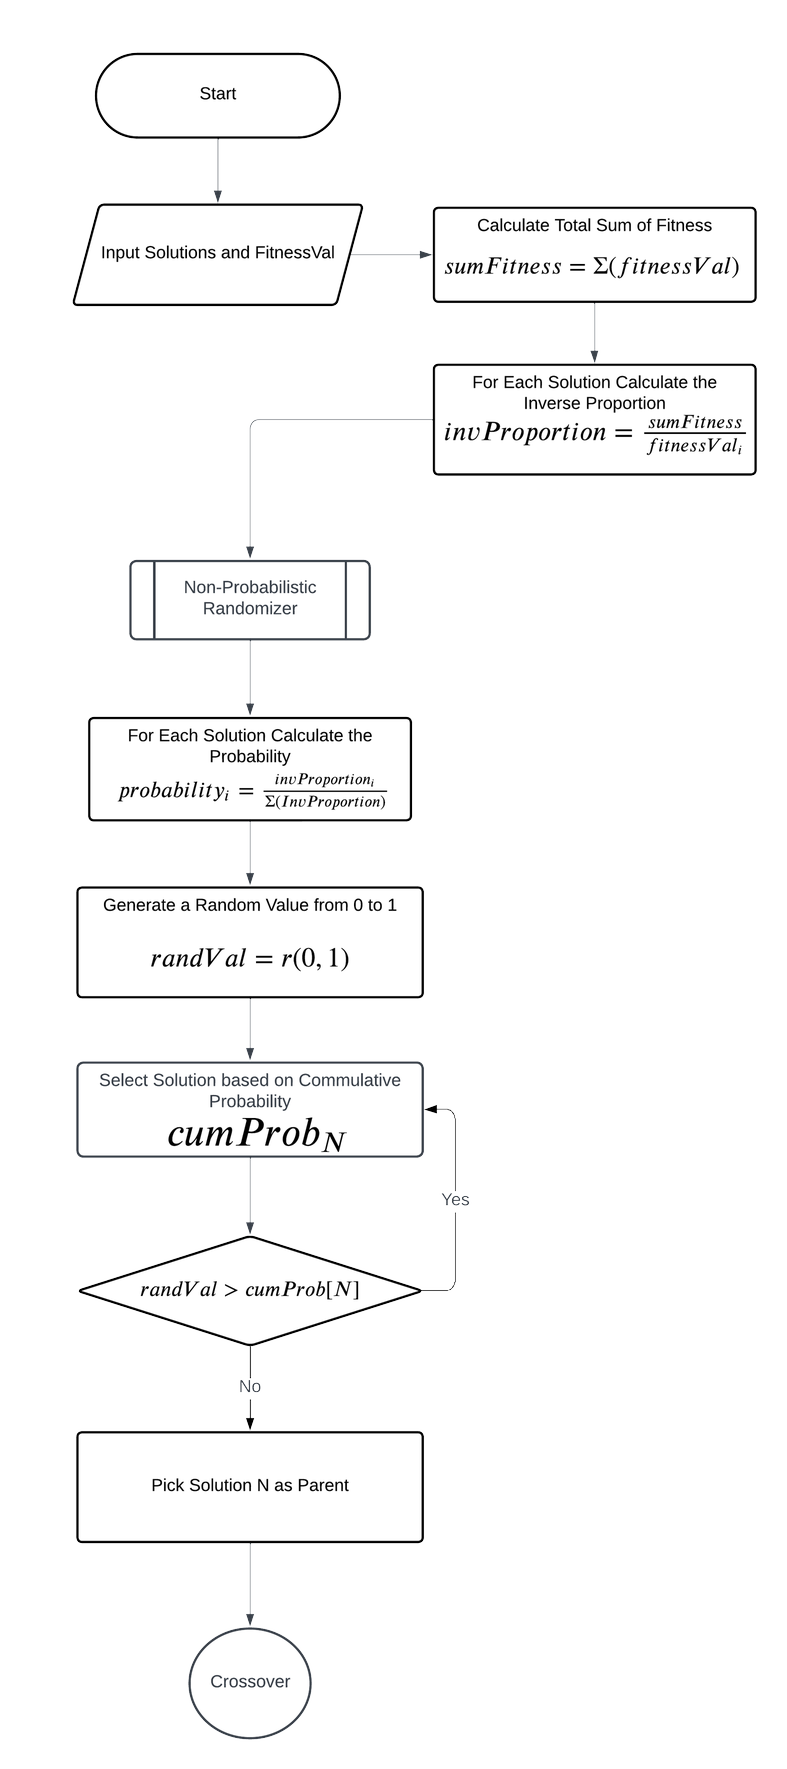
\includegraphics[width=\textwidth,height=\textheight,keepaspectratio]{appendix/select f}
		\end{figure}
		
		\begin{figure}[h]
			\centering
			\caption{Genetic Algorithm - Crossover}
			\label{crossFlow}
			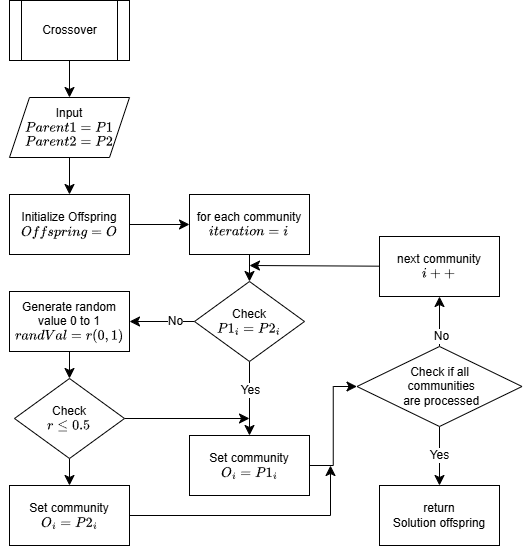
\includegraphics[width=\textwidth,height=\textheight,keepaspectratio]{appendix/crossover f}
		\end{figure}
		
		\begin{figure}[h]
			\centering
			\caption{Genetic Algorithm - Mutation}
			\label{mutateFlow}
			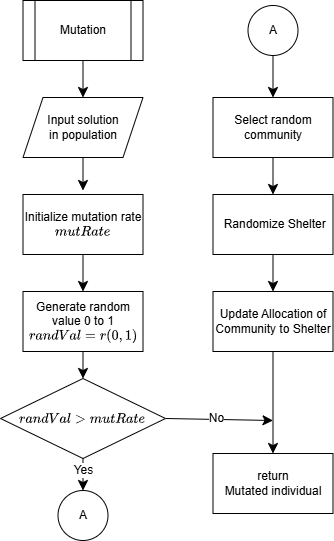
\includegraphics[width=\textwidth,height=\textheight,keepaspectratio]{appendix/mutate f}
		\end{figure}
		
		\begin{figure}[h]
			\centering
			\caption{Data Modification Feature}
			\label{dataModifFlow}
			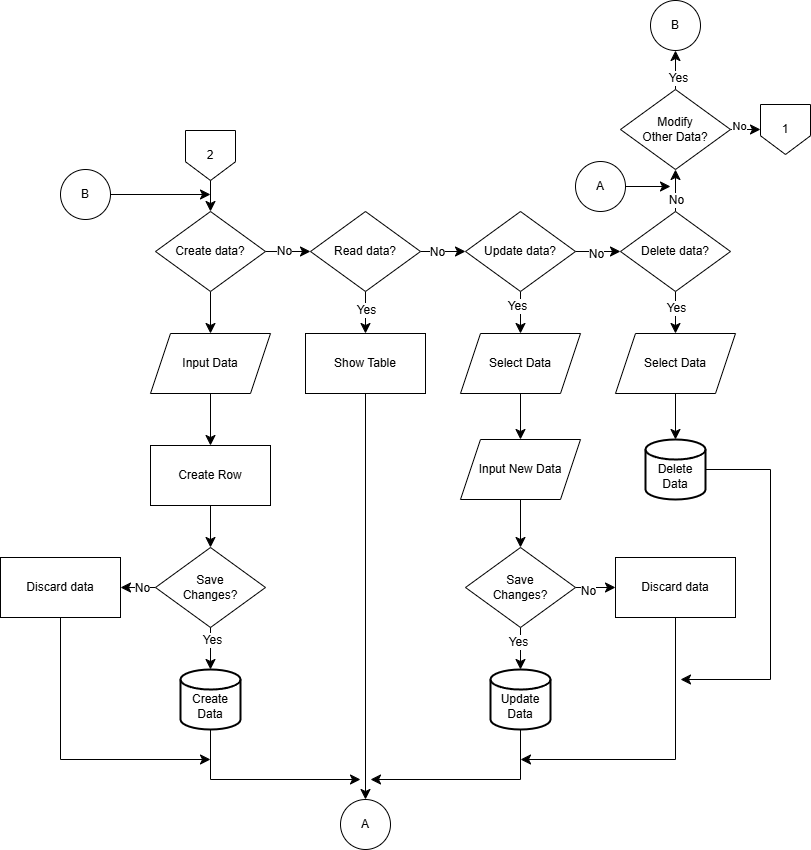
\includegraphics[width=\textwidth,height=\textheight,keepaspectratio]{appendix/data modif f}
		\end{figure}
		
		\begin{figure}[h]
			\centering
			\caption{Model Modification Feature}
			\label{modelFLow}
			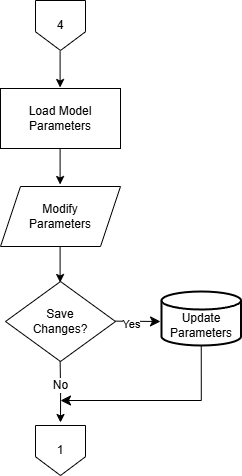
\includegraphics[width=\textwidth,height=\textheight,keepaspectratio]{appendix/modelset f}
		\end{figure}
		
		\begin{figure}[h]
			\centering
			\caption{Data Simulation Feature}
			\label{simFlow}
			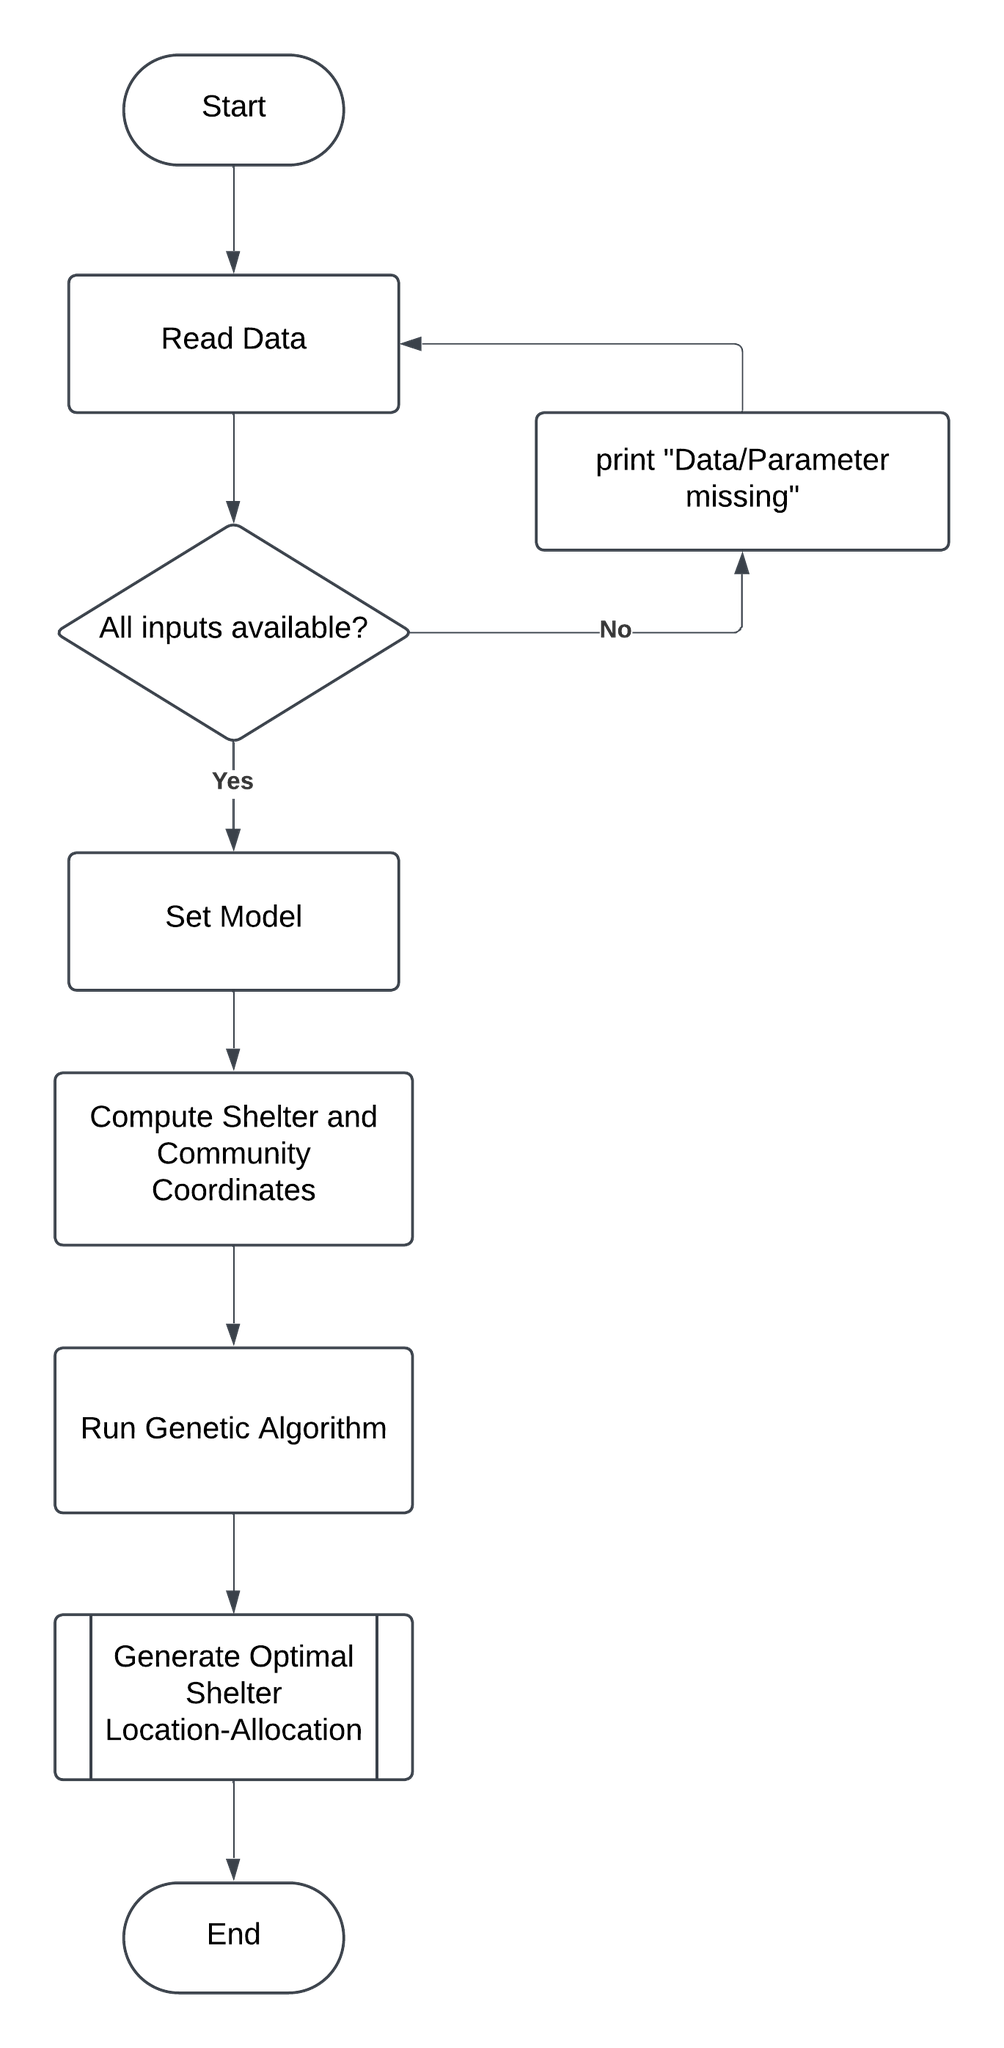
\includegraphics[width=\textwidth,height=\textheight,keepaspectratio]{appendix/datasim f}
		\end{figure}
		
		\begin{figure}[h]
			\centering
			\caption{Shelter Tagging Feature}
			\label{shelTagFlow}
			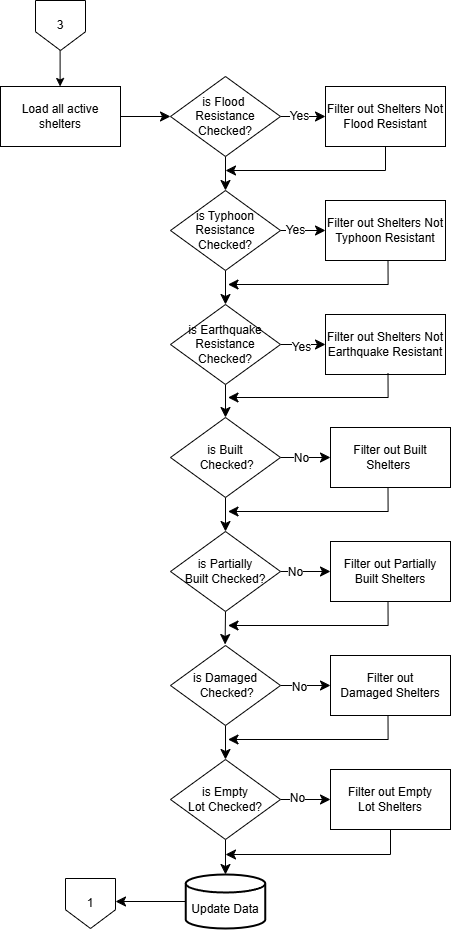
\includegraphics[width=\textwidth,height=\textheight,keepaspectratio]{appendix/sheltertag f}
		\end{figure}
		
		\begin{figure}[h]
			\centering
			\caption{Report Protection Feature}
			\label{protectFlow}
			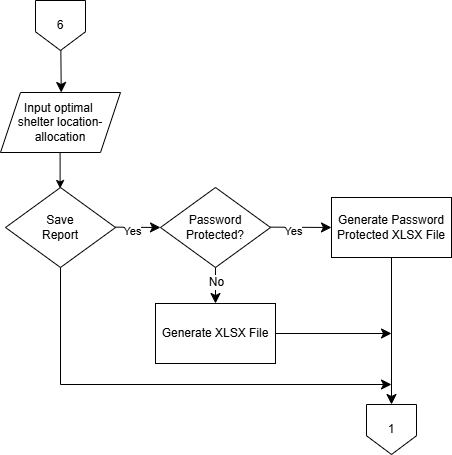
\includegraphics[width=\textwidth,height=\textheight,keepaspectratio]{appendix/protect f}
		\end{figure}
		
		
		
	\end{centerappendixtitle}
	
	\begin{centerappendixtitle}
		% use centerappendixtitle if the supplementary materials will cover the entire page
		% input the title as usual then insert \pagebreak right after the title
		\chapter{Relevant Codes}
		\pagebreak
		
		
		\begin{lstlisting}[language=Python, caption={Genetic Algorithm}, label={genalgoCode}, breaklines=true]
 generation_last_updated = 0

 for _ in range(num_solutions):
     solution = spawn()
     solutions.append(solution)

 # generations
 for generation in range(num_generations):
     # check for cancellation
     if self.cancelled:
         self.progress_dialog("Genetic algorithm cancelled.")
         return

     # sorting from best to worst solutions
     ranked_solutions = [(fitness(sol), sol) for sol in solutions]
     ranked_solutions.sort(key=lambda x: x[0]) aaaaaaaaaaaaaaaaaaaaaaaaaaaaaaaaaaaaaaaaaaaaaaaaaaa

     # initiate selection and crossover
     new_population = []
     for i in range(num_solutions):
         mother = selectParent(ranked_solutions)[1]
         father = selectParent(ranked_solutions)[1]

         offspring = generate_offspring(mother, father)
         new_population.append(offspring)

     # initiate mutation
     mutated_population = []
     for solution in new_population:
         if random.random() < mutation_rate:
             solution = mutate(solution)
         mutated_population.append((fitness(solution),solution))

     # getting the top half solutions
     best_solutions = mutated_population + ranked_solutions
     best_solutions = sorted(best_solutions, key=lambda x: x[0])[:num_solutions] 

     if (generation+1) % 100 == 0 :
         self.progress_dialog(str(best_solutions[0]))
         print(best_solutions[0])
         self.progress_dialog(f"=== Gen {generation+1} best solution ===")
         print(f"=== Gen {generation+1} best solution ===")

     prev_best_solution = fitness(solutions[0])

     # replace old population
     solutions = [sol[1] for sol in best_solutions]

     new_best_solution = fitness(solutions[0])

     #update generation_last_updated
     if(prev_best_solution != new_best_solution):
         generation_last_updated = generation+1
\end{lstlisting}
		
\begin{lstlisting}[language=Python,caption={Genetic Algorithm - Selection}, label={selectionCode}]
def selectParent(solutions):
	sum_fitness = sum(fitness for fitness, _ in solutions)
	inv_proportions = [sum_fitness/ fitness for fitness, _ in solutions]
	sum_inv_proportions = sum(inv_proportions)
	probability = [inv_proportion / sum_inv_proportions for inv_proportion in inv_proportions]
	solution_indices = np.arange(len(solutions))
	
	selected_solution = np.random.choice(solution_indices, p=probability)
	
	return solutions[selected_solution]
\end{lstlisting}

\begin{lstlisting}[language=Python,caption={Genetic Algorithm - Crossover}, label={crossoverCode}]
def generate_offspring(parent1, parent2):
    offspring = {"initial":{},"shelterlvl":{}}
    for community in Community:
        #for initial
        shelters = {parent1["initial"][community["name"]], parent2["initial"][community["name"]]} 
        
        if shelters:
            chosen_shelter = random.choice(list(shelters))
        else:
            chosen_shelter = random.choice([shelter["name"] for shelter in Shelters])

        offspring["initial"][community["name"]] = chosen_shelter

    for shelter in Shelters:

        #for shelterlvl
        levels = {parent1["shelterlvl"][shelter["name"]], parent2["shelterlvl"][shelter["name"]]} 
        
        if shelters:
            chosen_lvl = random.choice(list(levels))
        else:
            chosen_lvl = random.choice([1,2])

        offspring["shelterlvl"][shelter["name"]] = chosen_lvl

    return offspring
\end{lstlisting}

\pagebreak
\begin{lstlisting}[language=Python,caption={Genetic Algorithm - Mutation}, label={mutationCode}]
def mutate(allocation):
    new_allocations = copy.deepcopy(allocation)

    for _ in range(mutation_iteration) : 
        key_rand = random.choice(list(allocation.keys()))
        gene_to_mutate = random.choice(list(allocation[key_rand].keys()))
        current_value = allocation[key_rand][gene_to_mutate]
        
        if key_rand == "initial" or key_rand == "transferred":
            available_choices = [shelter["name"] for shelter in Shelters if shelter["name"] != current_value]
        elif key_rand == "shelterlvl":
            available_choices = [1,2]
            available_choices.remove(current_value)

        if available_choices:
            new_value = random.choice(available_choices)
            new_allocations[key_rand][gene_to_mutate] = new_value
            
    return new_allocations
\end{lstlisting}

\pagebreak
\begin{lstlisting}[language=Python,caption={Objective Value}, label={objValCode}]
def fitness(allocation):
    initial_shelters = set(allocation['initial'].values())
    Shelters_dict = {shelter["name"]: shelter for shelter in Shelters}

    total_distance = 0
    total_cost = 0

    for community in Community:
        # add distance * population
        shelter_name = allocation["initial"][community["name"]]
        distance = community["distances"][shelter_name]
        total_distance += distance * community["population"]


    for shelter_name in initial_shelters:
        # add cost based on shelter level
        shelter = Shelters_dict.get(shelter_name)
        if (allocation["shelterlvl"][shelter_name] == 1):
            total_cost += shelter["cost1"] 
        elif (allocation["shelterlvl"][shelter_name] == 2):
            total_cost += shelter["cost2"] 
        else:
            print("Shelter exceeded 2 levels. Something is wrong")
        
    # the actual model
    objective_value = weight_dist * total_distance + weight_cost * total_cost
    penalty_value = penalty_constant * getPenaltySum(allocation)

    # handle division by zero
    if objective_value + penalty_value == 0:
        return 1

    return int(objective_value + penalty_value)
\end{lstlisting}

\begin{lstlisting}[language=Python,caption={Maximum Distance Constraint}, label={maxdistCode}]
def check_max_distance(allocation):
    penalty = 0

    for community in Community:
        shelter_name = allocation["initial"][community["name"]]
        distance = community["distances"][shelter_name]
        max_distance_community = community["maxdistance"]
        # check if distance is greater than max dist
        if (distance > max_distance_community):
            print("maximum distance constraint failed")
            penalty += distance - max_distance_community
        
    return penalty
\end{lstlisting}

\pagebreak
\begin{lstlisting}[language=Python,caption={Capacity Constraint}, label={capCode}]
def check_initial_capacity(allocation):
    shelter_areas = {shelter["name"]: shelter[f"area{allocation["shelterlvl"][shelter['name']]}"] for shelter in Shelters}
    used_area = {shelter["name"]: 0 for shelter in Shelters}

    penalty = 0

    for community in Community:
        shelter_name = allocation["initial"][community["name"]]
        if shelter_name:
            # add to used_area based on population
            required_area = community["population"] * area_per_individual
            used_area[shelter_name] += required_area

            if used_area[shelter_name] > shelter_areas[shelter_name]:
                print("initial capacity constraint failed")

    for shelter in Shelters:
        shelter_name = shelter["name"]
        penalty_value = used_area[shelter_name] - shelter_areas[shelter_name]
        penalty += max(0,penalty_value)

    return penalty
\end{lstlisting}

\begin{lstlisting}[language=Python,caption={Maximum Shelter Constraint}, label={maxshelCode}]
def check_max_shelters(allocation):
    used_shelters = set() 
    penalty = 0

    for community in Community:
        shelter_name = allocation["initial"][community["name"]]
        used_shelters.add(shelter_name)  

    # If the number of unique shelters exceeds the max allowed
    if len(used_shelters) > max_shelters:
        print("max shelters constraint failed")
        penalty += len(used_shelters) - max_shelters
            
    return penalty
\end{lstlisting}

\pagebreak
\begin{lstlisting}[language=Python,caption={Maximum Level 2 Shelter Constraint}, label={maxl2shelCode}]
def check_max_lvl2_shelters(allocation):
    lvl2_shelters_ctr = sum(1 for level in allocation["shelterlvl"].values() if level == 2)
    penalty = 0

    if lvl2_shelters_ctr > max_lvl2_shelters:
        print("max lvl2 shelters constraint failed")
        penalty += lvl2_shelters_ctr - max_lvl2_shelters 

    return penalty
\end{lstlisting}
		
		
		
	\end{centerappendixtitle}
	
	\begin{centerappendixtitle}
		% use centerappendixtitle if the supplementary materials will cover the entire page
		% input the title as usual then insert \pagebreak right after the title
		\chapter{Letters}
		\pagebreak
		
		
\includepdf[pages=1,pagecommand={}]{appendix/Letter-of-Intent-Research-Collab-MDRRMO-Participants}
		
\includepdf[pages=1,pagecommand={}]{appendix/Letter-of-Intent-Research-Collab-MSWDO-Participants}
		\includepdf[pages=-,pagecommand={}]{appendix/Thesis-Endorsement}
		
		
	\end{centerappendixtitle}
	
	\begin{centerappendixtitle}
		% use centerappendixtitle if the supplementary materials will cover the entire page
		% input the title as usual then insert \pagebreak right after the title
		\chapter{Questionnaires}
		\pagebreak
		
		
		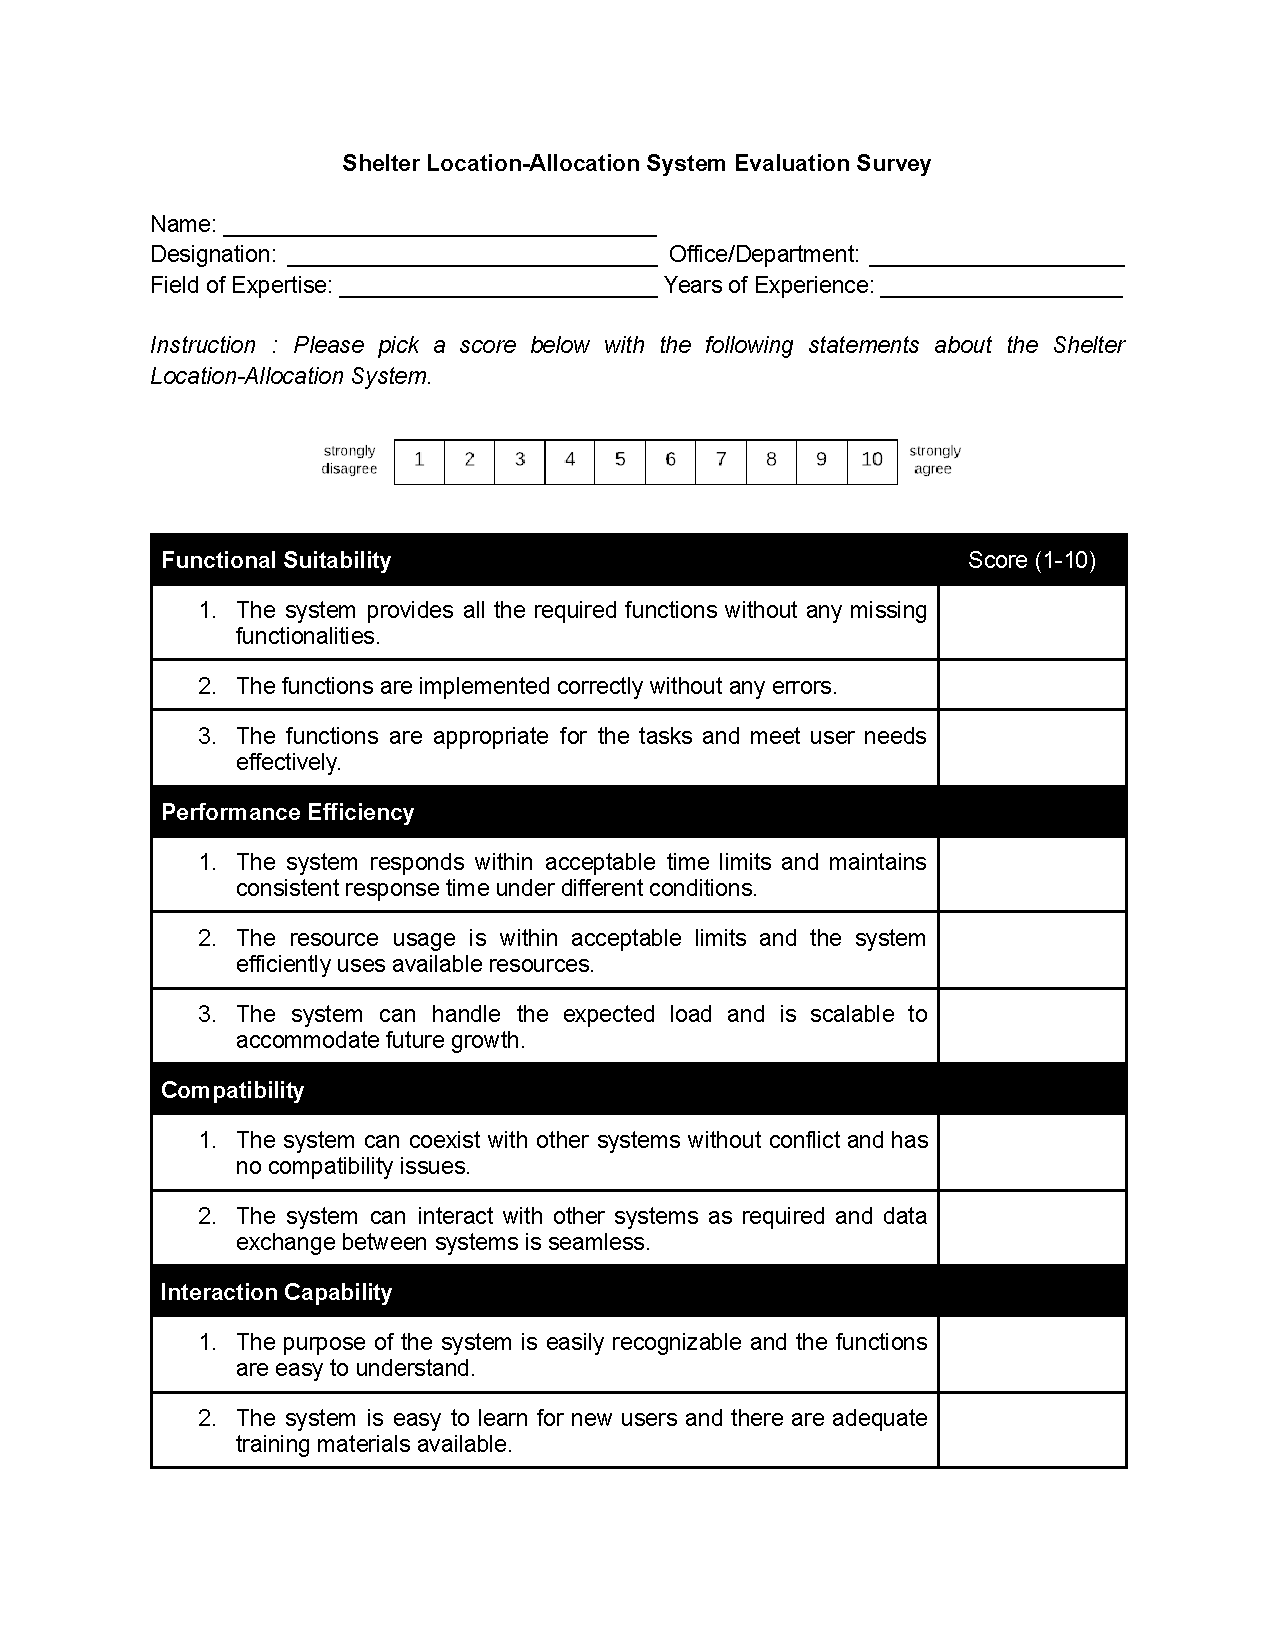
\includepdf[pages=-,pagecommand={}]{appendix/[ISOQuestionnaire]_Thesis}
		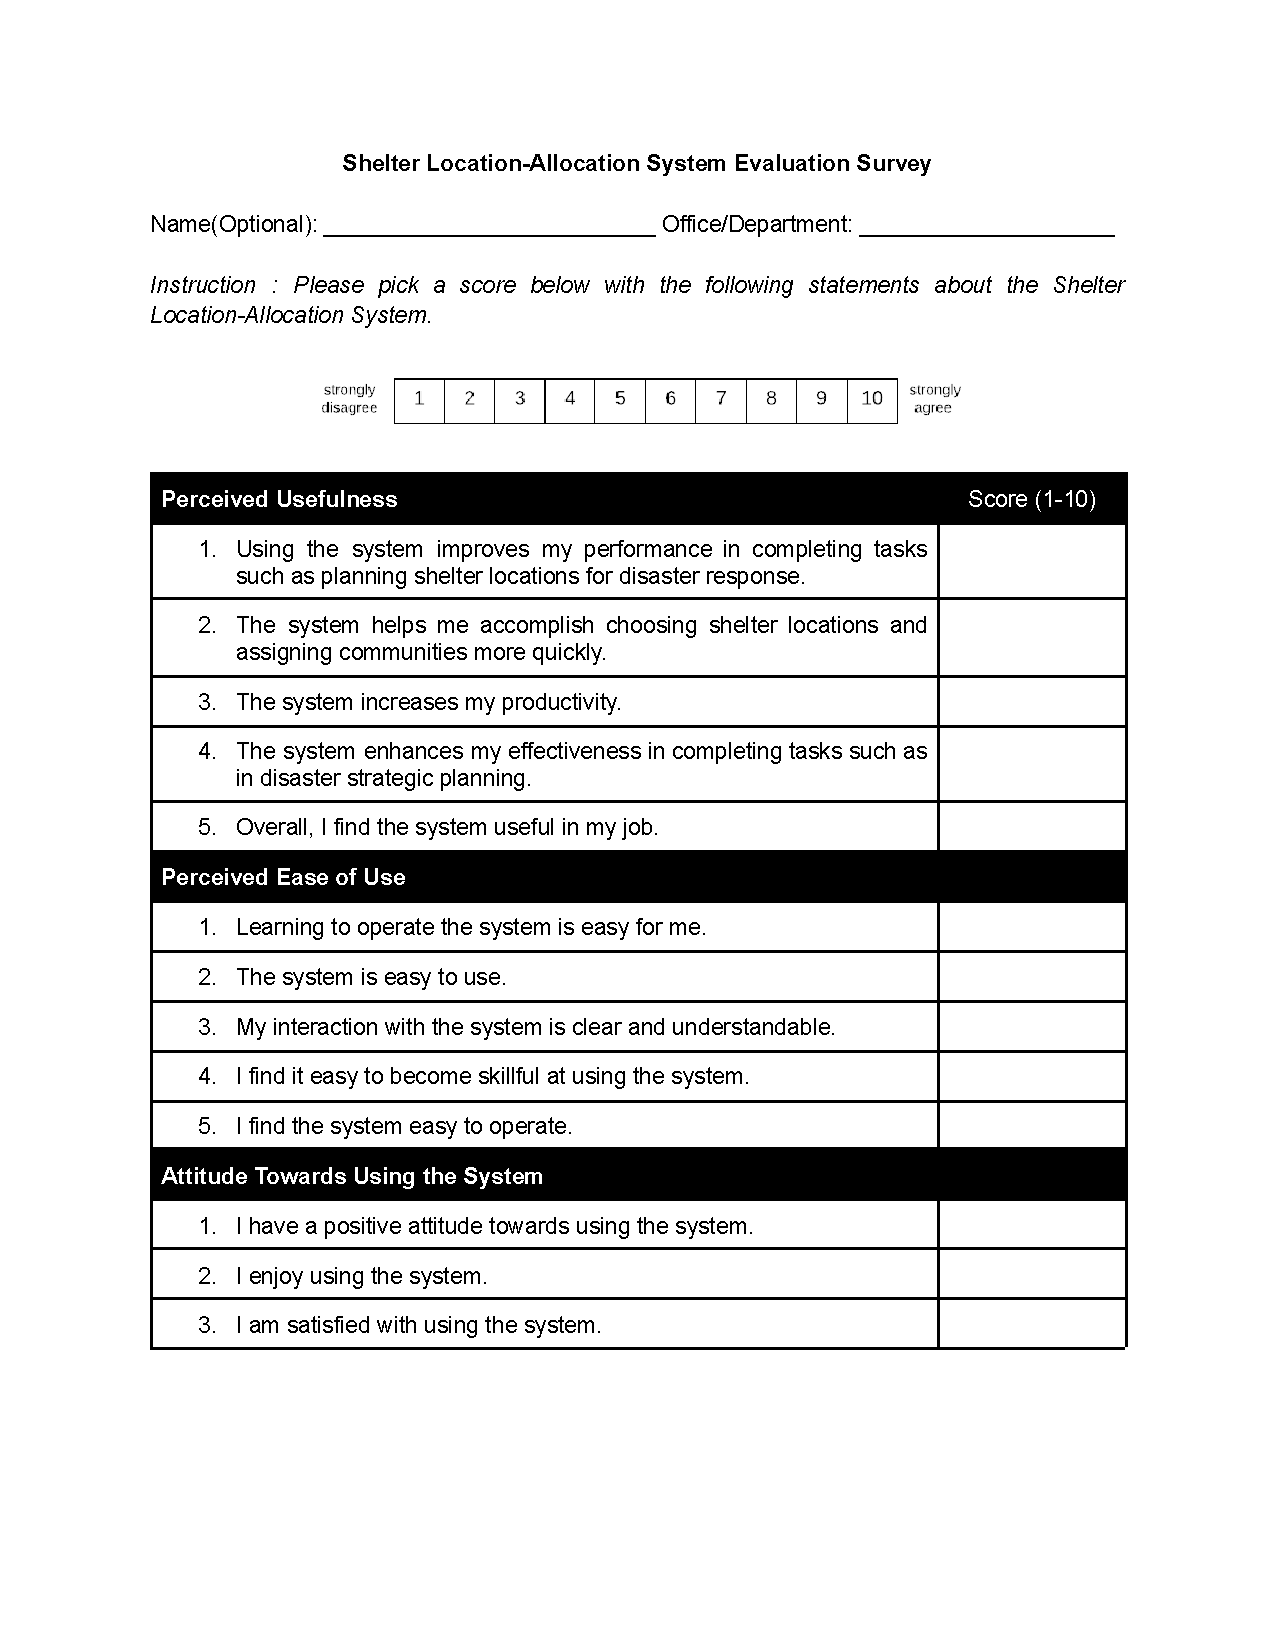
\includepdf[pages=-,pagecommand={}]{appendix/[TAMQuestionnaire]_Thesis}
	\end{centerappendixtitle}
	
	
	
\end{appendices}